%!TEX root = presentation.tex

% memo: mille modi per centrare
% https://tex.stackexchange.com/questions/449578/basic-how-can-i-stop-centering-a-text

\subsection{Introduction}

\begin{frame}{Outline}
    Situation calculus provides a framework for reasoning about actions.

    This work presents an expansion to handle the \textit{knowledge} possessed or acquired by the agent,
    and allow it to shape the agent's decisions.
    \begin{itemize}%[<+->]
        \item Knowledge is represented by one additional fluent
        \item Uniform axiomatization with the rest of sitcalc
        \item Ordinary actions and knowledge-producing ones are strictly separated
        \item Easy expansion of regression as defined in [Reiter2001]
        \item Desirable properties are direct consequences of the axiomatization \\
                (e.g. knowledge persistence / memory)
    \end{itemize}
\end{frame}

% opzionale
% \begin{frame}{...}
%     Opzionale

%     Un paio di azioni ordinarie e un paio di azioni di conoscenza di esempio, giusto per inquadrare il discorso
% \end{frame}

\subsection{Knowledge as a fluent}

\begin{frame}[fragile]{The K fluent}
    \huge
    \[ \sck(s', s) \]
    \normalsize

    Defines an accessibility relation between situations.

    \begin{block}{(Informal) definition}
        \( \sck(s',s) \) is true if an agent in situation \(s\)
        could mistake the current situation for the other \(s'\),
        given its current knowledge.
    \end{block}
\end{frame}

\begin{frame}{Knowledge}
    \begin{block}{Definition of knowledge}
        A fluent is known to be true (false) in a situation \(s\)
        if and only if it is true (false)
        in all situations accessible from \(s\).
    \end{block}

    Shorthand notation: \( \knows(\phi, s) \defeq \forall s' \: \sck(s',s) \rightarrow \phi(s') \)
\end{frame}

\begin{frame}{Knowledge-producing actions}
    Actions that have an effect on the agent's knowledge

    \begin{block}{SENSE actions}
        Learn the truth value of a formula. Example: check if a door is open or closed.
        \[
            \knows(\scp, \scdo(\scsense_{\scp}, s))
            \lor
            \knows(\lnot \scp, \scdo(\scsense_{\scp}, s))
        \]
    \end{block}

    \begin{block}{READ actions}
        Learn the value of a term. Example: read a number on a sheet of paper.
        \[
            \exists x \: \knows(\tau = x, \scdo(\scread_\tau, s))
        \]
    \end{block}

    % \emph{Assumption: ordinary and knowledge-producing actions are strictly separated.}
\end{frame}

\subsection{Defining a successor state axiom for K}

\begin{frame}{Knowledge effects}
    In order to complete the specification of the \sck{} fluent,
    we need to define its successor state axiom,
    determining how ordinary actions and knowledge-producing actions affect it.

    Consider this case study with three accessible situations. The agent is in S1.

    \begin{center}
        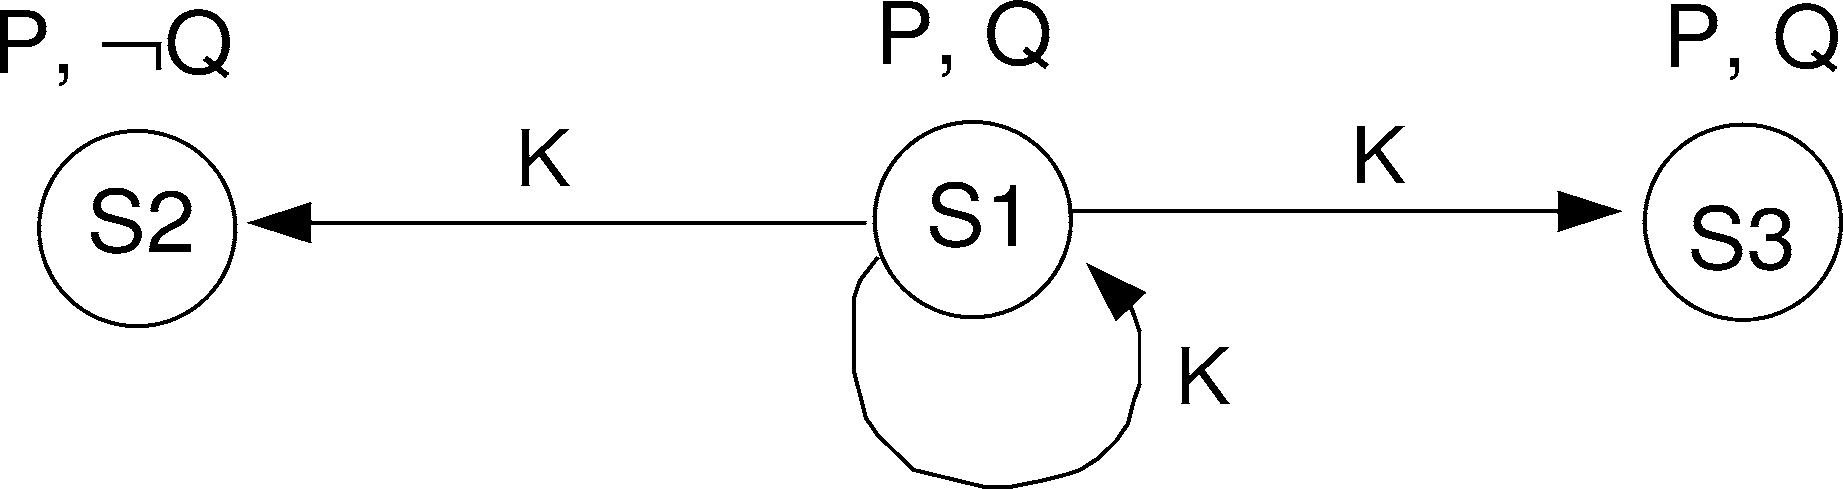
\includegraphics[width=0.6\textwidth]{assets/3states_noactions.png}
    \end{center}

    \[ \knows(\scp, S1) \land \lnot \knows(\scq, S1) \]
\end{frame}

\begin{frame}{Ordinary actions}
    Assume the agent performs a \textfluent{drop} action.

    \begin{block}{Informal idea}
        The agent cannot distinguish the current situation \(s\) from all the other
        \(s'\) accessible from it. Therefore, after executing the action,
        the agent may believe to be in any situation resulting from any \(s'\) after executing \scdrop.
    \end{block}

    \begin{block}{Axiomatization}
        \[ \sck(s'', \scdo(\scdrop, s)) \equiv \exists s' \: (\scposs(\scdrop, s') \land \sck(s',s) \land s'' = \scdo(\scdrop, s')) \]
    \end{block}
\end{frame}

\begin{frame}{Ordinary actions}
    \begin{columns}
        \begin{column}{0.5\textwidth}
            The \textbf{only knowledge gained is that the} \scdrop{} \textbf{action has been performed},\\
            as well as anything that can be derived from the action effects.
            
            For example, if \scdrop{} makes \scp{} false:

            \[ \scp(\scdo(a,s)) \equiv a \not = \scdrop \land \scp(s) \]

            then

            \[ \knows(\lnot \scp, \scdo(\scdrop, S1)) \]

            but no extra knowledge is gained about \scq.
        \end{column}

        \begin{column}{0.5\textwidth}
            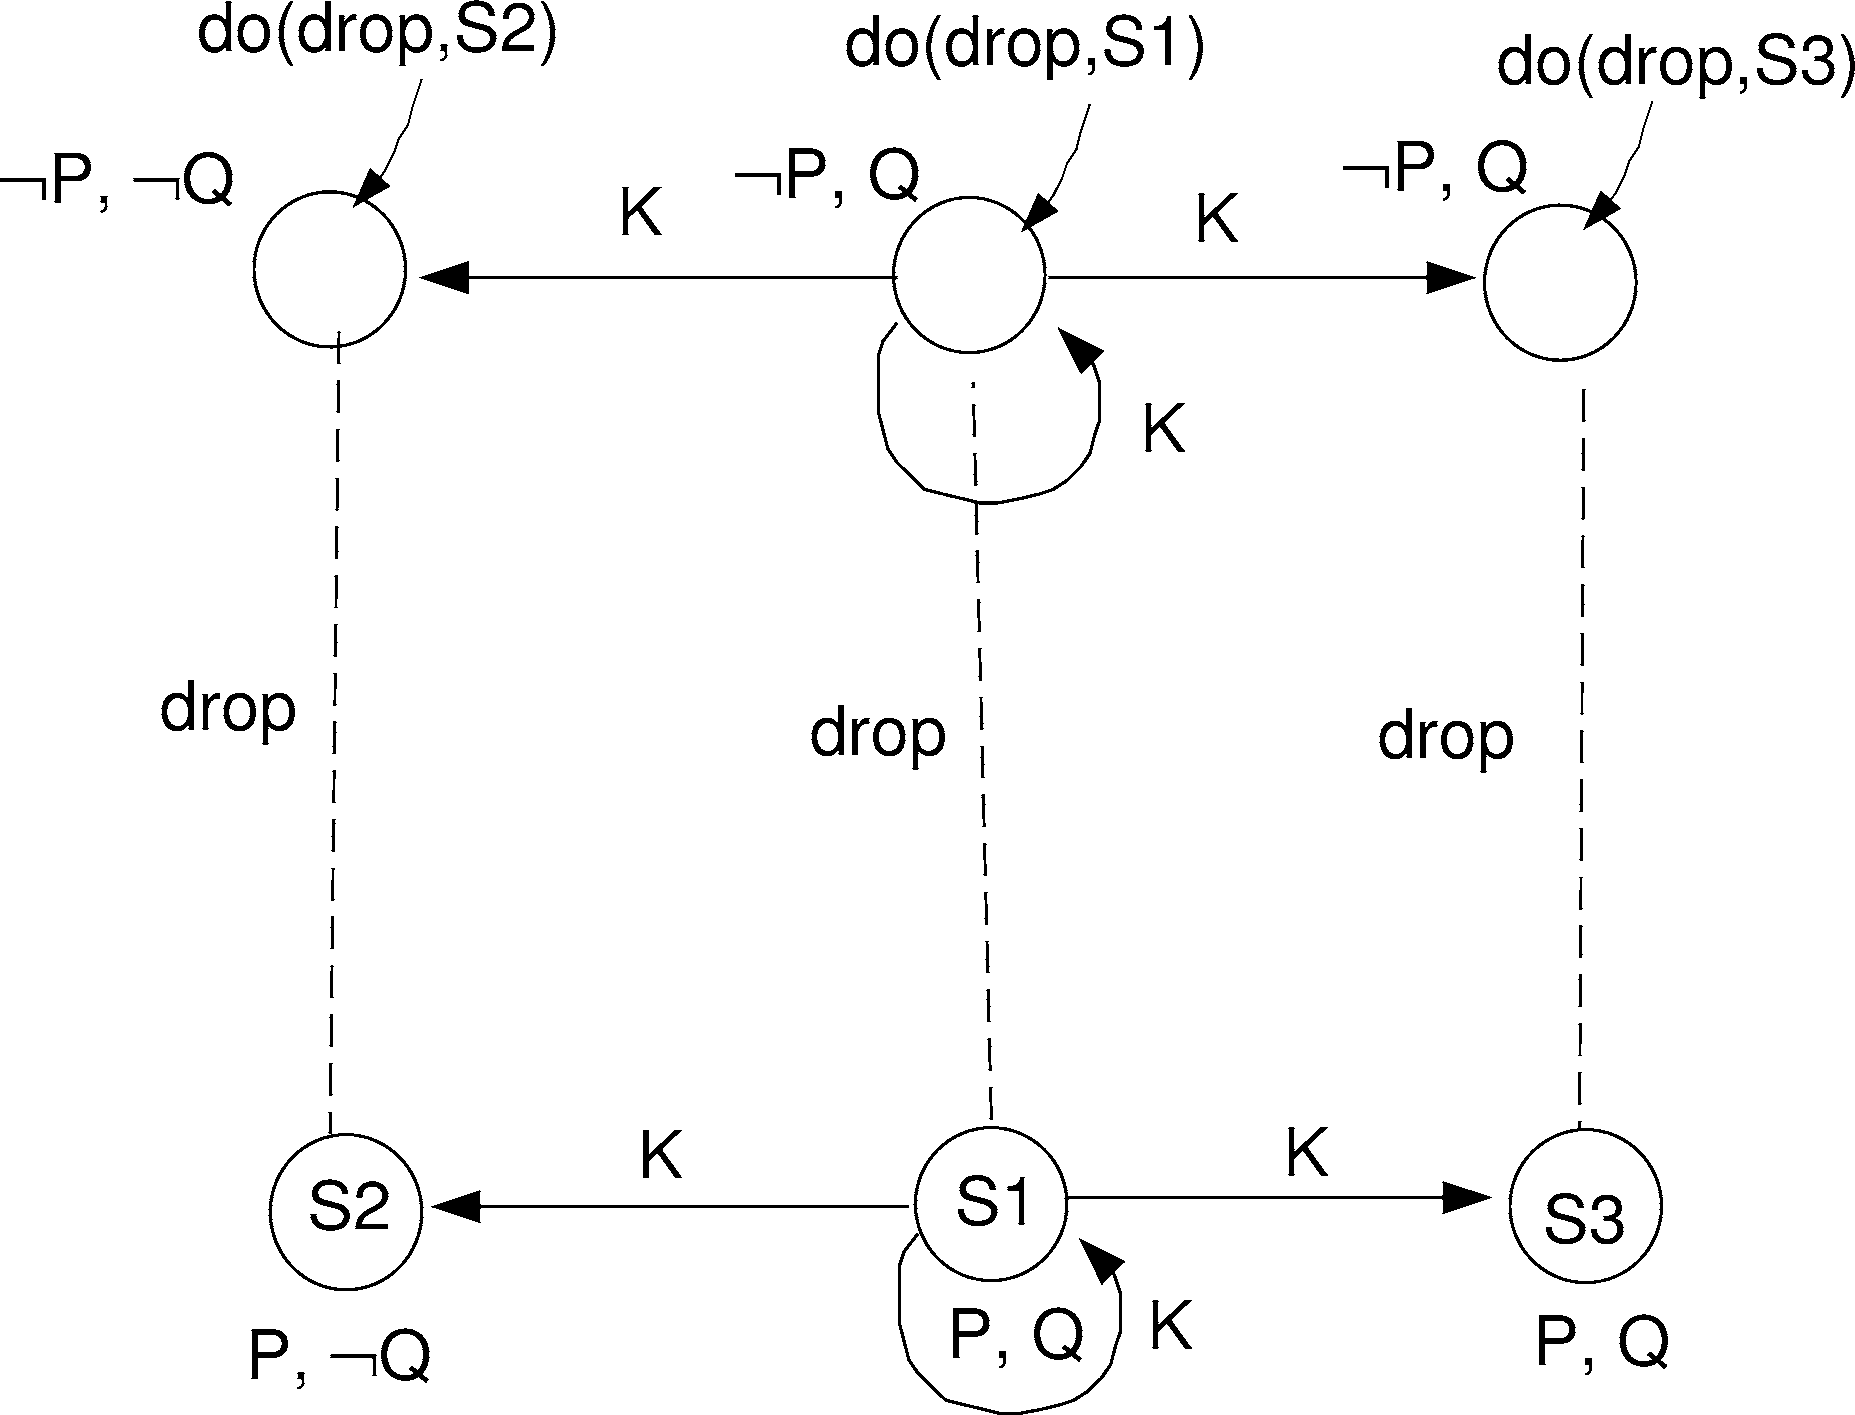
\includegraphics[width=\textwidth]{assets/3states_dropaction}
        \end{column}
    \end{columns}
\end{frame}

\begin{frame}{Knowledge-producing actions}
    Consider an action \( \scsense_{\scq} \) that provides information on whether \scq{} is true or false.

    We define a \textbf{sensing result function} to represent the signal received by the agent in response:

    \begin{block}{Sensing result function}
        \[ \scsr(\scsense_{\scq}, s) = r \equiv (r = \scyes \land \scq(s)) \lor (r = \scno \land \lnot \scq(s)) \]
    \end{block}
\end{frame}

\begin{frame}{Knowledge-producing actions}
    \vspace{-0.2cm}
    When the agent executes \( \scsense_{\scq} \), what are the accessible situations afterwards?

    \begin{block}{Informal definition}
        Initially, the agent cannot distinguish the current situation \(s\) from all the other
        \(s'\) accessible from it. Therefore, after executing \( \scsense_{\scq} \),
        the agent may believe to be in any situation that:
        \begin{itemize}
            \item results from any \(s'\) after executing the action,
            \item \textbf{AND} would yield the same sensing result as the one that has been observed.
        \end{itemize}
    \end{block}

    \begin{block}{Axiomatization}
        \vspace{-0.5cm}
        \begin{align*}
            \sck(s'', \scdo(\scsense_{\scq}, s)) \equiv \: & \exists s' \: (\scposs(\scsense_{\scq}, s') \land \sck(s',s) \: \land \\
            & s'' = \scdo(\scsense_{\scq}, s') \land \scsr(\scsense_{\scq}, s) = \scsr(\scsense_{\scq}, s'))
        \end{align*}
    \end{block}
\end{frame}

\begin{frame}{Knowledge-producing actions}
    \begin{columns}
        \begin{column}{0.5\textwidth}
            After executing \( \scsense_{\scq} \),
            \textbf{only situations with the same truth value for Q are accessible}.

            Thus, in addition to knowing that \( \scsense_{\scq} \) has been performed,
            the agent now knows the truth value of \scq{} as well, by definition.

            \[ \knows(\scq, \scdo(\scsense_{\scq}, S1)) \]
        \end{column}

        \begin{column}{0.5\textwidth}
            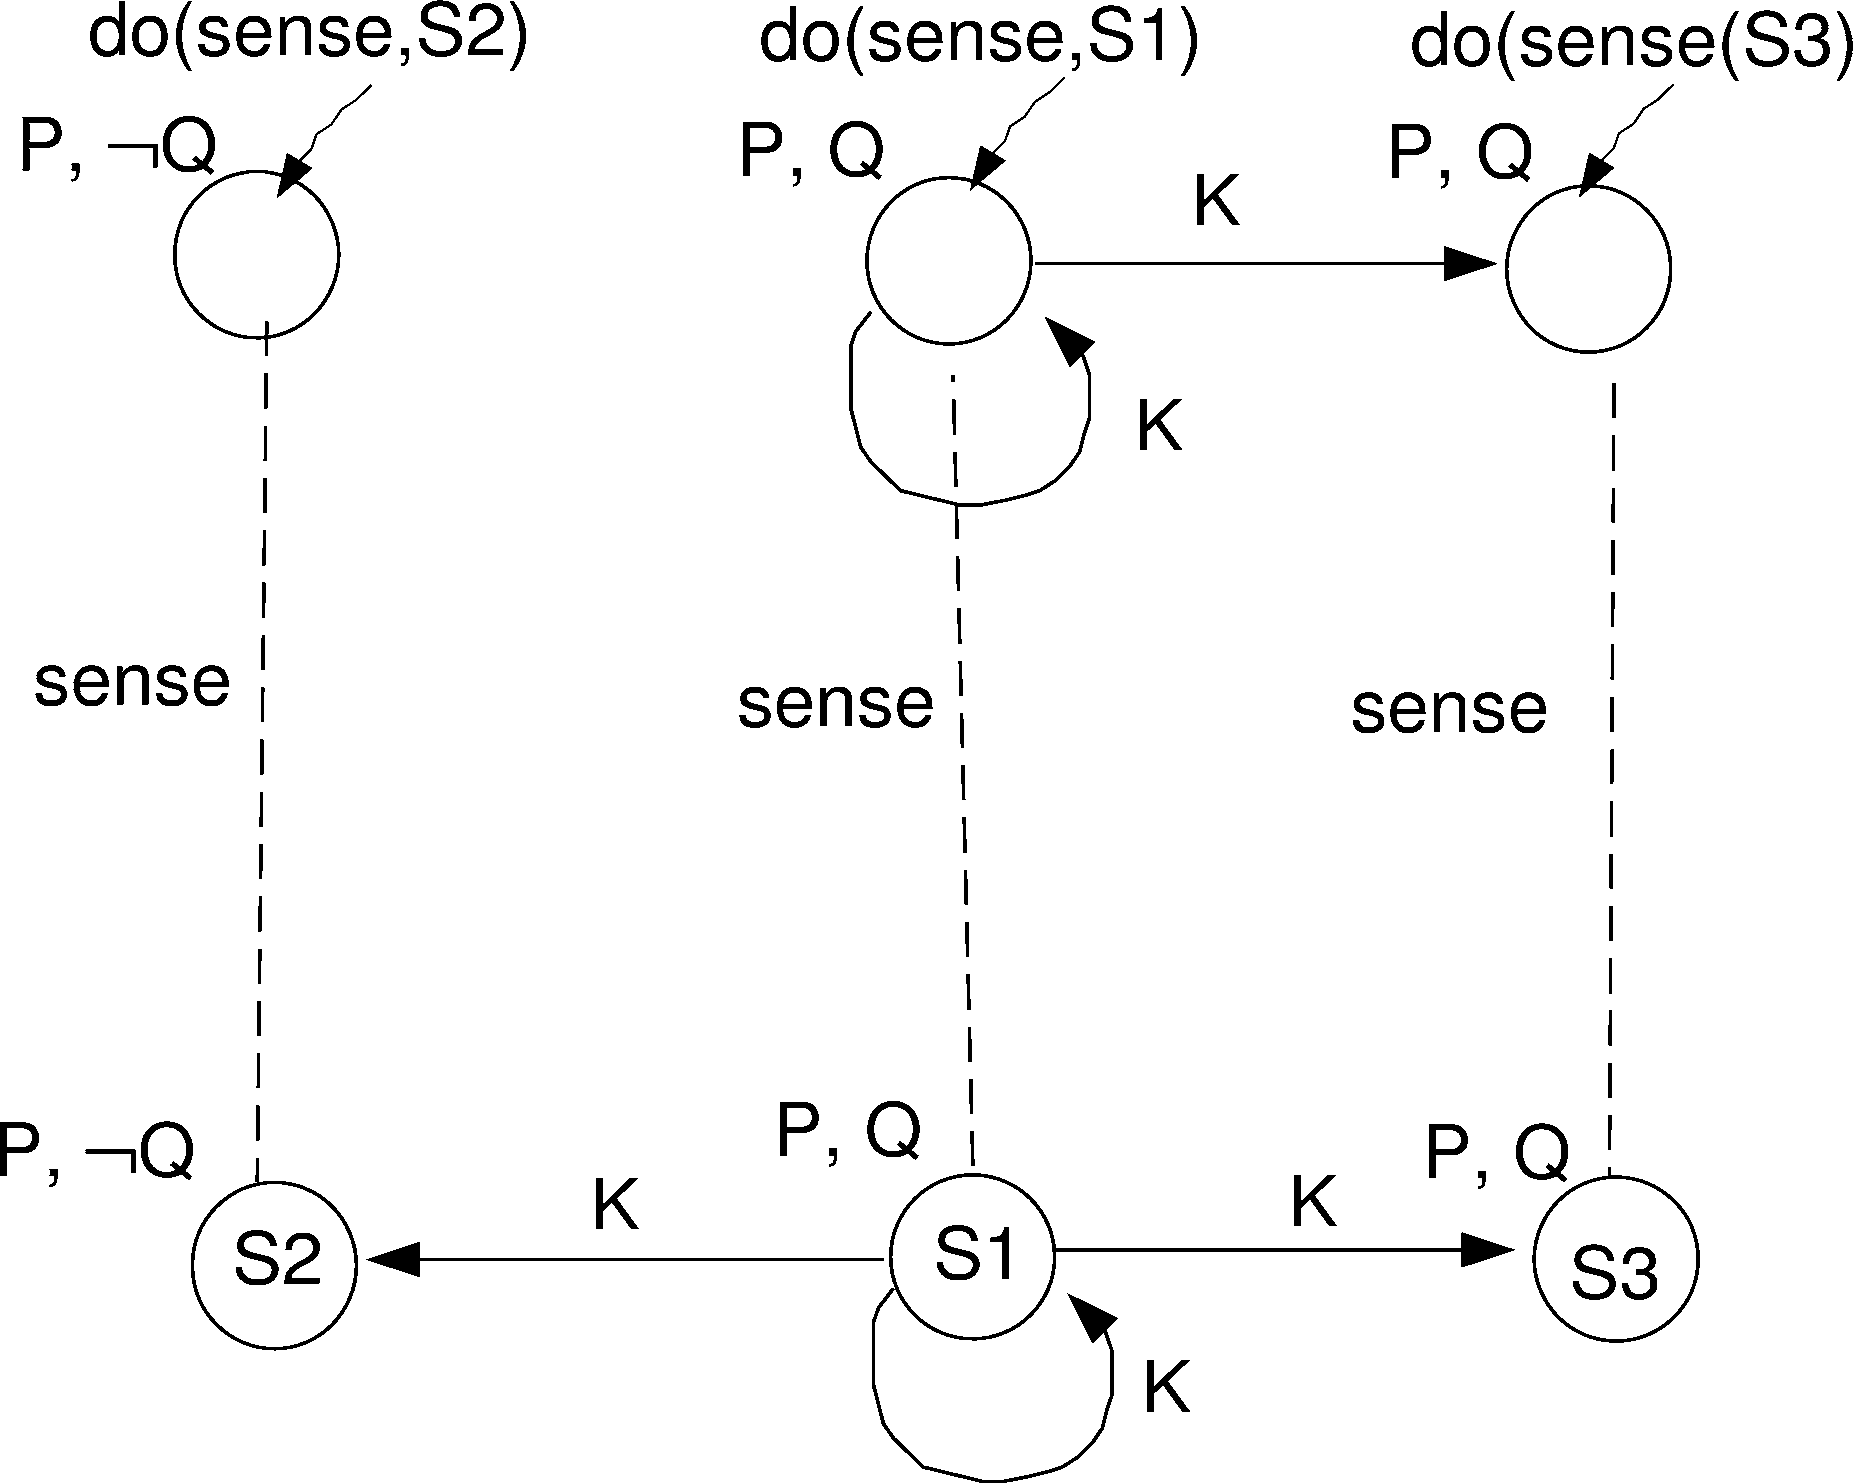
\includegraphics[width=\textwidth]{assets/3states_senseaction}
        \end{column}
    \end{columns}
\end{frame}

\begin{frame}{Sensing results in general}
    The concept of sensing result extends to all types of action, allowing for a uniform axiomatization.

    \begin{block}{Ordinary actions}
        \[ \scsr(\scdrop, s) = r \equiv r = \scok \]
    \end{block}

    \begin{block}{SENSE-type knowledge-producing actions}
        \[ \scsr(\scsense_{\scq}, s) = r \equiv (r = \scyes \land \scq(s)) \lor (r = \scno \land \lnot \scq(s)) \]
    \end{block}

    \begin{block}{READ-type knowledge-producing actions}
        \[ \scsr(\scsense_\tau, s) = r \equiv r = \tau(s) \]
    \end{block}
\end{frame}

\begin{frame}{The successor state axiom for K}
    Putting it all together, the definitive form is as follows:

    \begin{block}{Successor state axiom for the K fluent}
        \vspace{-0.5cm}
        \begin{align*}
            \sck(s'', \scdo(a, s)) \equiv \exists s' \: (&\scposs(a, s') \land \sck(s',s) \: \land \\
            & s'' = \scdo(a, s') \land \scsr(a, s) = \scsr(a, s'))
        \end{align*}
    \end{block}
\end{frame}

\begin{frame}{What about...}
    \begin{itemize}
        \item \textbf{...mixing ordinary and knowledge effects?} \\
            We assume that ordinary and knowledge actions are disjoint:
            each action is going to be axiomatized
            as either affecting \emph{only} the \sck{} fluent
            or as not affecting it at all. \\
            This does not cause loss of generality.
        \item \textbf{...knowledge of arbitrary formulae?} \\
            They already work within this system. \\
            Example: \( \knows(\forall x (\textfluent{man}(x) \rightarrow \textfluent{mortal}(x)) \land \textfluent{man}(Socrates)) \)
    \end{itemize}
\end{frame}

% \begin{frame}{<varie ed eventuali>}
%     boh
% \end{frame}
